\documentclass[12pt, twoside]{article}
\usepackage[letterpaper, margin=1in, headsep=0.5in]{geometry}
\usepackage[english]{babel}
\usepackage[utf8]{inputenc}
\usepackage{amsmath}
\usepackage{amsfonts}
\usepackage{amssymb}
\usepackage{tikz}
\usetikzlibrary{quotes, angles}
\usepackage{graphicx}
\usepackage{enumitem}
\usepackage{multicol}

\newif\ifmeta
\metatrue %print standards and topics tags

\title{Regents Geometry}
\author{Chris Huson}
\date{January 2022}

\usepackage{fancyhdr}
\pagestyle{fancy}
\fancyhf{}
\renewcommand{\headrulewidth}{0pt} % disable the underline of the header
\raggedbottom

\fancyhead[LE]{\thepage}
\fancyhead[RO]{\thepage \\ Name: \hspace{4cm} \,\\}
\fancyhead[LO]{BECA / Dr. Huson / Geometry 6 Trigonometry}

\begin{document}
\subsubsection*{6.10 Classwork: Tangent applications \hfill CCSS.HSG.SRT.C.8}
Write an equation expressing $\tan \theta$ as a ratio of \emph{opposite} over \emph{adjacent}, then solve for the missing length.
\begin{enumerate}
\item Do Now: Given right $\triangle JKL$ with $\overline{JK} \perp \overline{KL}$, $JK=8$, $m\angle J=24^\circ$. Let $x$ be the length of the side opposite $\angle J$, $x=KL$.
    \begin{flushright}
        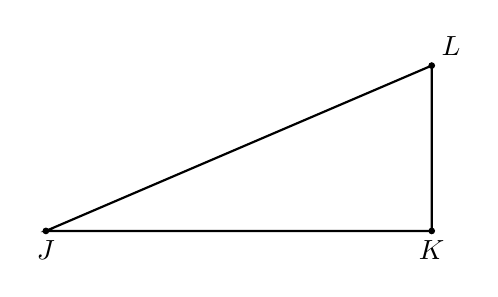
\begin{tikzpicture}[scale=0.7]
          \draw [thick](-1,0)--(6,0)--(6,3)--cycle;
          \draw [fill] (-1,0) circle [radius=0.05] node[below]{$J$};
          \draw [fill] (6,0) circle [radius=0.05] node[below]{$K$};
          \draw [fill] (6,3) circle [radius=0.05] node[above right]{$L$};
        \end{tikzpicture}
      \end{flushright} \vspace{1.5cm}

\item $\triangle ABC$ is shown with $m\angle C=90^\circ$ and the lengths of the triangle's sides are $BC=8$, $AC=15$, and $AB=17$.  \hfill (not drawn to scale)
\begin{multicols}{2}
      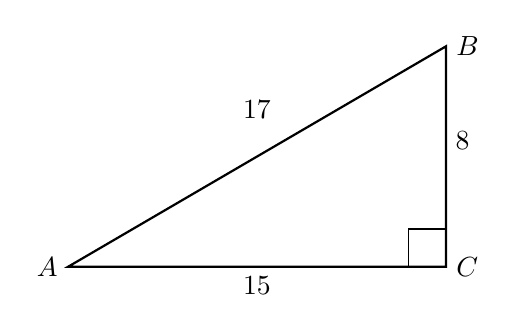
\begin{tikzpicture}[scale=0.8]
        \draw [thick]
        (0,0)node[left]{$A$}--
        (6,0)node[ right]{$C$}--
        (6,3.5)node[right]{$B$}--cycle;
        \draw (6,0)++(-0.6,0)--++(0,0.6)--+(0.6,0);
        \node at (3,0)[below]{$15$};
        \node at (6,2)[right]{$8$};
        \node at (3,2.2)[above]{$17$};
      \end{tikzpicture}
      \begin{enumerate}
      \item Write down the value of $\tan A$. \vspace{1.25cm}
      \item Find the measure of $\angle A$.  \vspace{1cm}
    \end{enumerate}
  \end{multicols} %\vspace{2cm}

\item The diagram shows a building with observer $A$ on the ground looking up at $B$ on the building roof. Point $A$ is 40 feet from the building and the angle of elevation from $A$ to $B$ is $25^\circ$.\\[0.25cm]
Find the height of the building to the \emph{nearest foot}. \hfill (not drawn to scale)
  \begin{flushright}
    \begin{tikzpicture}[scale=0.4]
      %\draw [-, thick] (0,0)--(35:23);
      \draw [-, thick] (-4,0)--
      (0,0)--
        (17,0)--
        (22,0)--
        (22,10)--(17,10)--(17,0);
      \draw [fill] (0,0) circle [radius=0.1] node[above]{$A$};
      \draw [fill] (17,10) circle [radius=0.1] node[above right]{$B$};
      \draw [dashed] (0,0)--(17,10);
      \node at (3, 0)[above]{$25^\circ$};
      \node at (-3, 0)[above]{ground};
      \node at (19.5, 5)[above]{building};
    \end{tikzpicture}
    \end{flushright}
    
\newpage
\item From the top of a seaside cliff, a sailboat is visible at an angle of depression of $4^\circ$. If the cliff is 100 feet tall, determine the distance of the boat from shore, $x$, to the \emph{nearest foot}.
\begin{center}
    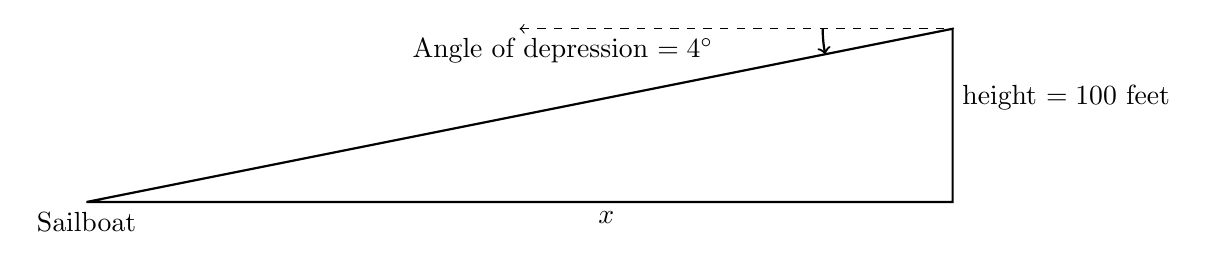
\begin{tikzpicture}[scale=1.1]
      \draw [thick] (10,0)--(0,0)--(10,2.0)--cycle;
      \draw [dashed, <-] (5,2)--(10,2.0);
      \draw [thick, ->] (8.5,2) arc [start angle=180, end angle=191.3, radius=1.5];
      \node at (5.5,2)[below]{Angle of depression $=4^\circ$};
      \node at (10,1.2)[right]{height $=100$ feet};
      \node at (6,0)[below]{$x$};
      \node at (0,0)[below]{Sailboat};
    \end{tikzpicture}
  \end{center} \vspace{3.25cm}

\item A zipline wire is strung from a pole to the ground with an angle of elevation of $12^\circ$. If the pole is 30 feet tall, how long is the wire, to the \emph{nearest foot}. \\[0.25cm]
(hint: first find the distance to the pole horizontally, then use the Pythagorean theorem to find the hypotenuse, the wire)\\[0.25cm]
  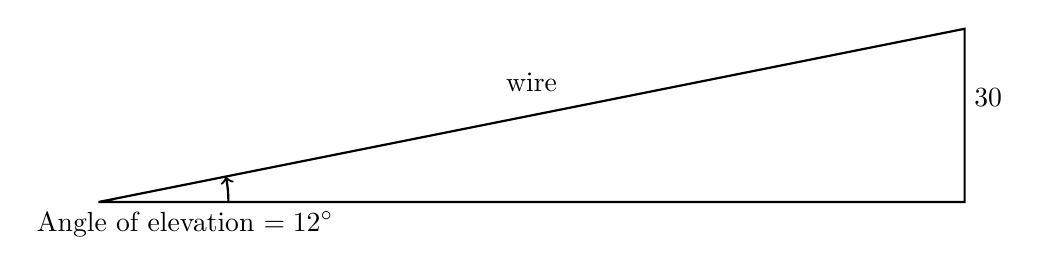
\begin{tikzpicture}[scale=1.1]
    \draw [thick] (10,0)--(0,0)--(10,2.0)--cycle;
    \draw [thick, ->] (1.5,0) arc [start angle=0, end angle=11.3, radius=1.5];
    \node at (1,0)[below]{Angle of elevation $=12^\circ$};
    \node at (10,1.2)[right]{$30$};
    \node at (5,1.6)[below]{wire};
  \end{tikzpicture} \vspace{4cm}

\end{enumerate}
\end{document}

\item A sailor observes the top of a lighthouse with an angle of elevation of $4^\circ$. She knows the lighthouse is 100 feet tall. Determine and state the distance $x$ between the sailor and the lighthouse, to the \emph{nearest foot}.\\[0.25cm]
    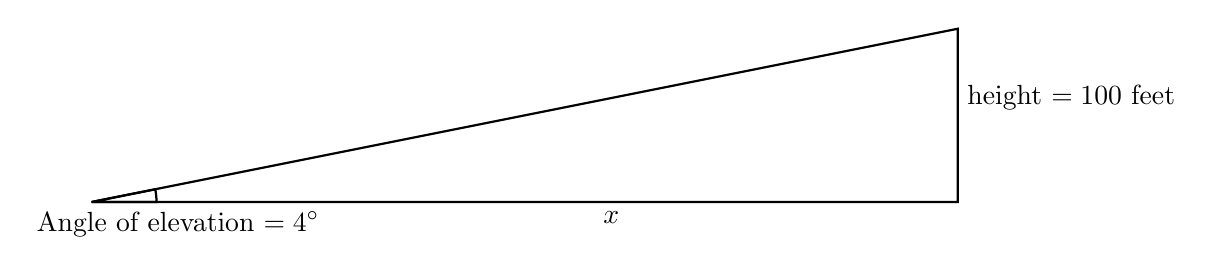
\begin{tikzpicture}[scale=1.1]
      \draw [thick] (10,0)--(0,0)--(10,2.0)--cycle;
      \draw [thick] (0,0)--(0.75,0) arc [start angle=0, end angle=11.3, radius=0.75]--cycle;
      \node at (1,0)[below]{Angle of elevation $=4^\circ$};
      \node at (10,1.2)[right]{height $=100$ feet};
      \node at (6,0)[below]{$x$};
    \end{tikzpicture} \vspace{3.25cm}

\item The following diagram shows a pole BT 1.6 m tall on the roof of a vertical building. \\[0.25cm]
The angle of elevation of the top of the building from A is  
$25^\circ$ and the distance from point $A$ to the building is 40 feet. (not drawn to scale)
  \begin{center}
    \begin{tikzpicture}[scale=0.4]
      %\draw [-, thick] (0,0)--(35:23);
      \draw [-, thick] (-4,0)--
      (0,0)--
        (17,0)--
        (22,0)--
        (22,10)--(17,10) node[left]{$B$};
      \draw [-, thick] (17,0)--(17,12)node[left]{$T$};
      \draw [fill] (0,0) circle [radius=0.1] node[below]{$A$};
      \draw [dashed] (0,0)--(17,10);
      \node at (3, 0)[above]{$25^\circ$};
      \node at (-3, 0)[below]{ground};
      \node at (19.5, 5)[above]{building};
    \end{tikzpicture}
    \end{center}
    Find the height of the building to the \emph{nearest foot}.